\clearpage
\begin{table}[H]\centering
\caption{All predefined controlled training runs}\label{tab:S15}
\small
\begin{tabular}{lrrrrrr}
\toprule
Configuration & Seed & Epoch & \shortstack{Internal\\AUROC} & \shortstack{External\\AUROC} & \shortstack{External\\sensitivity} & \shortstack{External\\specificity} \\
\midrule
Matched attention & 17 & 13 & \textbf{0.9314} & \underline{0.8170} & \textbf{80.26\%} & 62.50\% \\
Matched attention & 29 & 18 & \underline{0.9331} & \underline{0.7500} & \textbf{61.18\%} & 62.50\% \\
Matched attention & 43 & 12 & 0.9398 & 0.6139 & \textbf{34.87\%} & 56.25\% \\
\addlinespace
Fixed scaling & 17 & 24 & 0.9231 & \textbf{0.8701} & 53.29\% & \textbf{87.50\%} \\
Fixed scaling & 29 & 18 & \textbf{0.9431} & 0.7442 & 56.58\% & \underline{68.75\%} \\
Fixed scaling & 43 & 25 & \textbf{0.9532} & \underline{0.6192} & 13.16\% & \underline{62.50\%} \\
\addlinespace
Learned gate & 17 & 29 & \underline{0.9298} & 0.7311 & \underline{60.53\%} & \underline{68.75\%} \\
Learned gate & 29 & 20 & \underline{0.9331} & \textbf{0.9350} & \underline{59.21\%} & \textbf{93.75\%} \\
Learned gate & 43 & 29 & \underline{0.9431} & \textbf{0.6238} & \underline{17.76\%} & \textbf{68.75\%} \\
\addlinespace
\bottomrule
\end{tabular}
\par\medskip\raggedright\footnotesize Bold/underline compare configurations within the same seed and metric column. Each run used the same original 144/49 training/evaluation partition, 30 epochs, batch size eight, learning rate $5\times10^{-5}$, weight decay $10^{-4}$, dropout 0.3 and positive-class loss weight $77/67$. Within each seed, configurations shared identical initial values for common tensors, training bags and minibatch order. The original internal and external reference bags were fixed. Epoch denotes the first epoch with the highest internal AUROC; external evaluation was performed after selection. All nine predefined runs are reported. Matched attention shares the 256-dimensional projection, attention block and classifier construction but omits the other vectors, statistics and fusion layer. Fixed scaling multiplies all five vectors by 0.2; learned gating also changes nonlinear capacity. Parameters: matched attention 658,178, fixed scaling 1,190,403, learned gate 1,521,672. Thus these are controlled configuration comparisons, not parameter-matched or isolated single-component tests. Across-seed summaries describe training variation in the same cohort and do not add independent WSIs. No three-seed significance test is used. Source data: run\_metrics.csv, configuration\_summary.csv and paired\_seed\_differences.csv.
\end{table}

\begin{figure}[H]\centering
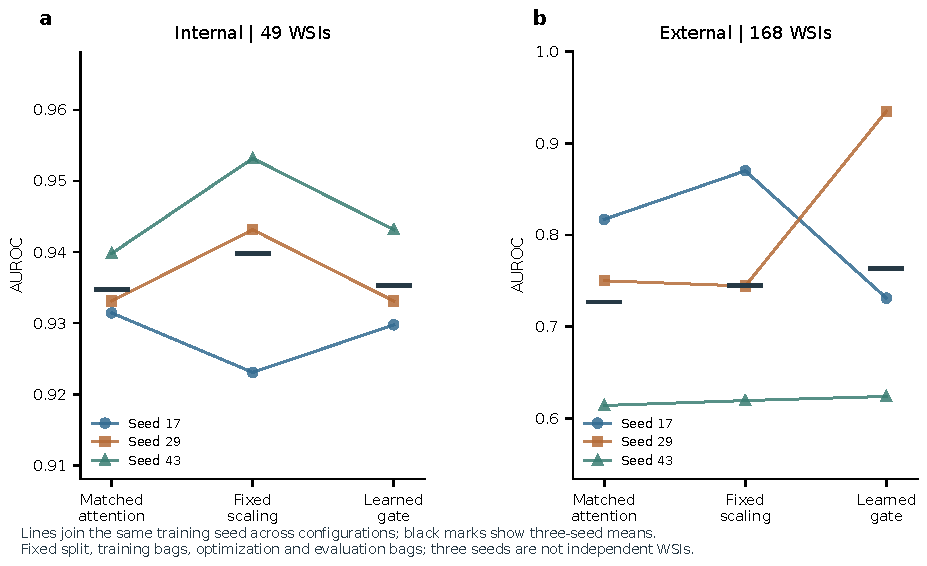
\includegraphics[width=\textwidth,height=.42\textheight,keepaspectratio]{figures/Supplementary_Figure_S4_controlled_training.pdf}
\caption{\textbf{Controlled configuration comparisons across three training seeds}. \textbf{a,b,} Internal and external AUROCs for every selected checkpoint from the nine predefined runs in Supplementary Table S15. Lines join the same seed across configurations and black horizontal marks denote three-seed means. Cohorts and evaluation inputs are unchanged across runs. Three seed values are descriptive training repeats rather than independent clinical observations; no confidence interval or inferential superiority claim is implied. Source data: run\_metrics.csv.}\label{fig:S4}
\end{figure}
